\newpage
\chapter{Theoretical Background -- Sensors \& PID}
\label{ap:b}

\section{Encoders}
\label{ap:b.enc}
A rotary encoder, also called a shaft encoder, is an electro-mechanical device that converts the angular position or motion of a shaft or axle to analog or digital output signals. There are two main types of rotary encoders: absolute and incremental. The output of an absolute encoder indicates the current shaft position, making it an angle transducer. The output of an incremental encoder provides information about the motion of the shaft, which typically is processed elsewhere into information such as position, speed, and distance.

\subsection{Technologies used in Encoders }
\begin{itemize}
    \item \textbf{Optical} 
    
    This uses a light shining onto a photodiode through slits in a metal or glass disc. Reflective versions also exist. This is one of the most common technologies. Optical encoders are very sensitive to dust. The resolutions of optical encoders are higher than magnetic encoders. 

    \item \textbf{On-Axis Magnetic}
    
    This technology typically uses a specially magnetized 2-pole neodymium magnet attached to the motor shaft. Because it can be fixed to the end of the shaft, it can work with motors that only have 1 shaft extending out of the motor body. The accuracy can vary from a few degrees to under 1 degree. Resolutions can be as low as 1 degree or as high as 0.09 degrees (4000 CPR). 

    \item \textbf{Off-Axis Magnetic} 
    
    This technology typically employs the use of rubber-bonded ferrite magnets attached to a metal hub. This offers flexibility in design and low cost for custom applications. Due to the flexibility in many off-axis encoder chips, they can be programmed to accept any number of pole widths so the chip can be placed in any position required for the application. Magnetic encoders operate in harsh environments where optical encoders would fail to work.
    
\end{itemize}

\subsection{Basic types}
\begin{itemize}
\item \textbf{Absolute}

This type maintains position information when power is removed from the encoder. The position of the encoder is available immediately on applying power. The relationship between the encoder value and the physical position of the controlled machinery is set at assembly; the system does not need to return to a calibration point to maintain position accuracy.

An absolute encoder has multiple code rings with various binary weightings which provide a data word representing the absolute position of the encoder within one revolution. This type of encoder is often referred to as a parallel absolute encoder. A multi-turn absolute rotary encoder includes additional code wheels and toothed wheels. A high-resolution wheel measures the fractional rotation, and lower-resolution geared code wheels record the number of whole revolutions of the shaft.

\item \textbf{Incremental}

This type will immediately report changes in position, which is an essential capability in some applications. However, it does not report or keep track of the absolute position. As a result, the mechanical system monitored by an incremental encoder may have to be homed (moved to a fixed reference point) to initialize absolute position measurements. We will discuss the concept of working on incremental encoders and why we used them in our project.
\end{itemize}

\subsection{Encoder Resolution Parameters}
\begin{itemize}
    \item \textbf{PPR(Pulses per Rotation):}
    describes the number of high pulses an encoder will have on either of its square waves outputs A or B over a single revolution. It is more common to represent the encoder resolution using PPR than CPR.

    \item \textbf{CPR(Counts per Rotation):}
    most commonly stands for Counts per Revolution, and refers to the number of quadrature decoded states that exist between the two outputs A and B. With both outputs A and B switching between high and low, there exist 2 bits of information represented as 4 distinct states. The term quadrature decoding describes the method of using both outputs A and B together to count each state change. This results in 4 times the number of counts that exist for each pulse or period. Therefore, the CPR of an encoder is the encoder’s PPR multiplied by 4.

\end{itemize}

\subsection{Encoder Working Principle}

The encoder has a disk with evenly spaced contact zones that are connected to the common pin C and two other separate contact pins A and B, as illustrated below.
\begin{figure}[h!]
     \centering
         \centering
         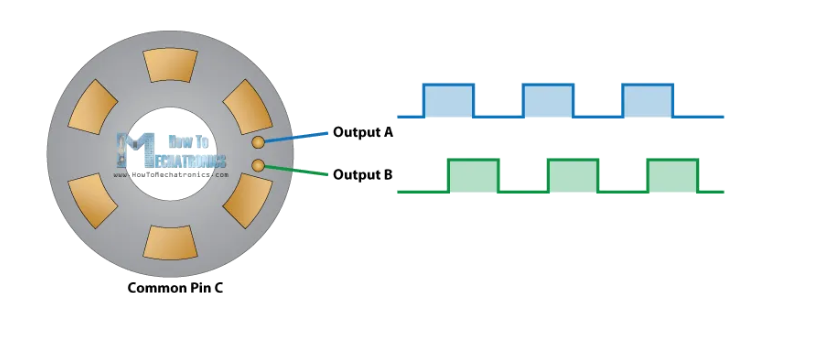
\includegraphics[scale=0.5]{./Figures/AppendixB/encoder.png}
         \caption{Pulses per Revolution Diagram}
         \label{fig: Pulses per Revolution Diagram}
\end{figure}
When the disk starts rotating step by step, the pins A and B will start making contact with the common pin and the two square wave output signals will be generated accordingly.

Any of the two outputs can be used for determining the rotated position if we just count the pulses of the signal. However, if we want to determine the rotation direction as well, we need to consider both signals at the same time.

We can notice that the two output signals are displaced at 90 degrees out of phase from each other. If the encoder is rotating clockwise output A will be ahead of output B. 
\begin{figure}[h!]
     \centering
         \centering
         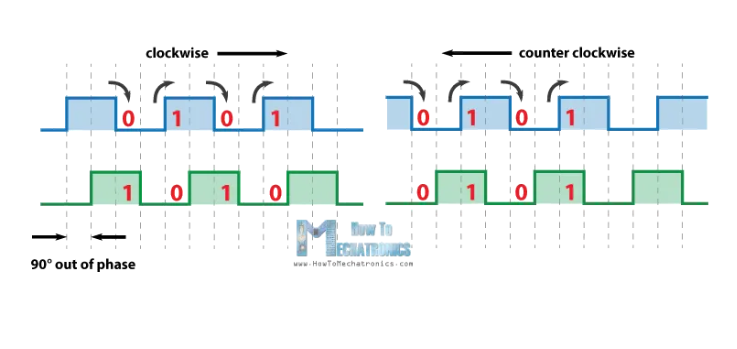
\includegraphics[scale=0.5]{./Figures/AppendixB/encoder-pulses.png}
         \caption{Encoder Output Signals}
         \label{fig: Encoder Output Signals}
\end{figure}
So if we count the steps each time the signal changes, from High to Low or from Low to High, we can notice that time the two output signals have opposite values. Vice versa, if the encoder is rotating counterclockwise, the output signals have equal values. So considering this, we can easily program our controller to read the encoder position and the rotation direction.





%%%%%%%%%%%%%%%%%%%%%%%%%%%%%%%%%%%

\section{IMU (Inertial Measurement Units)}
\label{ap:b.imu}
IMU sensors are based on multi-axis combinations of precision gyroscopes, accelerometers, magnetometers, and pressure sensors. its technology reliably senses and processes multiple degrees of freedom, even in highly complex applications and under dynamic conditions. These plugs-and-play solutions include full factory calibration, embedded compensation, and sensor processing, and a simple programmable interface. In our Project, we used MPU6050 IMU 

\subsection{MPU6050 Module}
The MPU6050 sensor module is a complete 6-axis Motion Tracking Device. It combines a 3-axis Gyroscope, 3-axis Accelerometer, and Digital Motion Processor all in a small package. Also, it has the additional feature of the on-chip Temperature sensor. It has an I2C bus interface to communicate with the microcontrollers.

It has an Auxiliary I2C bus to communicate with other sensor devices like 3-axis Magnetometer, Pressure sensor, etc.

If a 3-axis Magnetometer is connected to an auxiliary I2C bus, then MPU6050 can provide a complete 9-axis Motion Fusion output.
Let’s see MPU6050 inside sensors.

\begin{figure}[h!]
     \centering
         \centering
         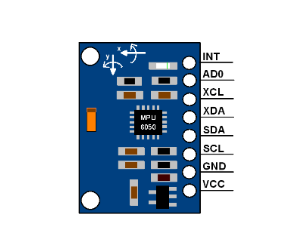
\includegraphics[scale=0.5]{./Figures/AppendixB/mpu.png}
         \caption{MPU6050 Module}
         \label{fig: MPU6050 Module}
\end{figure}

\begin{itemize}

    \item \textbf{3-Axis Gyroscope}
    
    The MPU6050 consists of a 3-axis Gyroscope with Micro Electro Mechanical System (MEMS) technology. It is used to detect rotational velocity along the X, Y, and Z axes as \ref{fig: MPU-6050 3-Axis Gyroscope}.
    
    \begin{figure}[h!]
         \centering
             \centering
             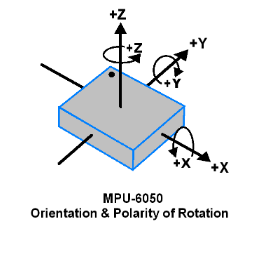
\includegraphics[scale=0.5]{./Figures/AppendixB/acc.png}
             \caption{MPU-6050 3-Axis Gyroscope}
             \label{fig: MPU-6050 3-Axis Gyroscope}
    \end{figure}


\begin{itemize}
        \item When the gyros are rotated about any of the sense axes, the Coriolis Effect causes a vibration that is detected by a MEM inside MPU6050.
        \item The resulting signal is amplified, demodulated, and filtered to produce a voltage that is proportional to the angular rate. 
        \item This voltage is digitized using 16-bit ADC to sample each axis.
        \item The full-scale range of output are +/- 250, +/- 500, +/- 1000, +/- 2000.
        \item It measures the angular velocity along each axis in degrees per second unit.
    \end{itemize}

    \item \textbf{3-Axis Accelerometer}
    
    The MPU6050 consists 3-axis Accelerometer with Micro Electro Mechanical (MEMs) technology. It is used to detect the angle of tilt or inclination along the X, Y, and Z axes as \ref{fig: MPU-6050 3-Axis Accelerometer}.
    
    \begin{figure}[h!]
     \centering
         \centering
         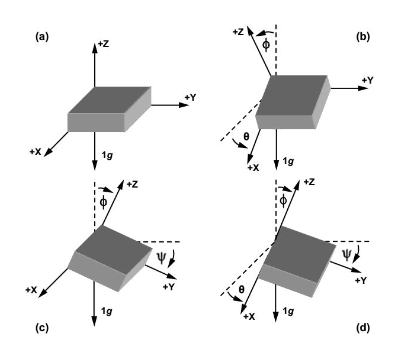
\includegraphics[scale=0.5]{./Figures/AppendixB/gyro.png}
         \caption{MPU-6050 3-Axis Accelerometer}
         \label{fig: MPU-6050 3-Axis Accelerometer}
         
    \end{figure}
    
    \begin{itemize}
        \item  Acceleration along the axes deflects the movable mass.
        \item This displacement of the moving plate (mass) unbalances the differential capacitor which results in sensor output. Output amplitude is proportional to acceleration.
        
        \item The full-scale range of acceleration are +/- 2g, +/- 4g, +/- 8g, +/- 16g.
        
        \item It measures in g (gravity force) unit.
        
        \item When the device is placed on a flat surface it will measure 0g on the X and Y axis and +1g on the Z axis.
    

    \end{itemize}

  \item \textbf{DMP (Digital Motion Processor)}
  
    The embedded Digital Motion Processor (DMP) is used to compute motion processing algorithms. It takes data from a gyroscope, accelerometer, and additional 3rd party sensors such as a magnetometer and processes the data. It provides motion data like roll, pitch, yaw angles, landscape portrait sense, etc. It minimizes the processes of the host in computing motion data. The resulting data can be read from DMP registers.
    
\end{itemize}
%%%%%%%%%%%%%%%%%%%%%%%%%%%%%%%%
\section{Ultrasonic}
    \label{ap:b.us}
An ultrasonic sensor is an electronic device that measures the distance of a target object by emitting ultrasonic sound waves and converts the reflected sound into an electrical signal. Ultrasonic waves travel faster than the speed of audible sound (i.e. the sound that humans can hear). 

Ultrasonic sensors have two main components: the transmitter (which emits the sound using piezoelectric crystals) and the receiver (which encounters the sound after it has traveled to and from the target).

\begin{figure}[h!]
     \centering
         \centering
         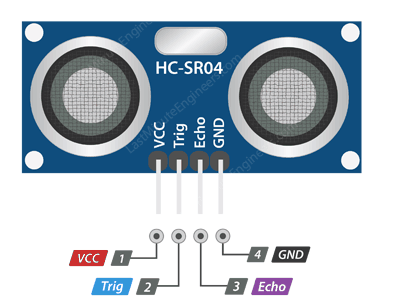
\includegraphics[scale=0.5]{./Figures/AppendixB/ulta2.png}
         \caption{Ultrasonic Module}
         \label{fig: Ultrasonic Module}
         
\end{figure}
To calculate the distance between the sensor and the object, the sensor measures the time it takes between the emission of the sound by the transmitter to its contact with the receiver. \\

The formula for this calculation is 
\[D = 0.5* T * C\] 

(where D is the distance, T is the time, and C is the speed of sound $\approx 343 m/s$). \\

For example, if a scientist set up an ultrasonic sensor aimed at a box and it took 0.025 seconds for the sound to bounce back, the distance between the ultrasonic sensor and the box would be:

$D = 0.5 * 0.025 * 343$
or about $4.2875m$.

\begin{figure}[h!]
     \centering
         \centering
         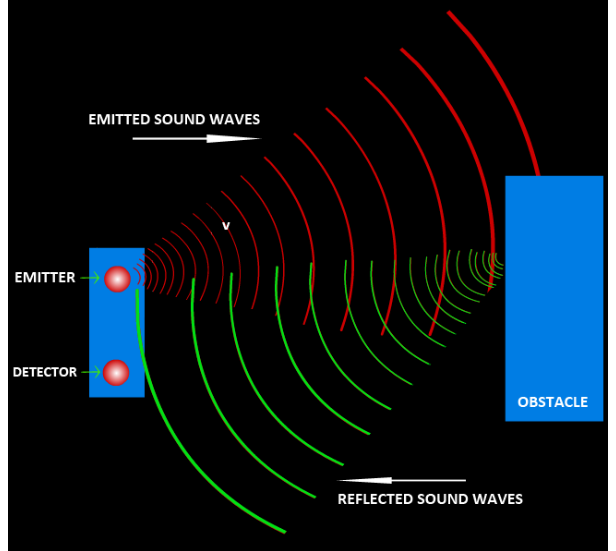
\includegraphics[scale=0.5]{./Figures/AppendixB/ultra1.png}
         \caption{Ultrasonic sensor diagram}
         \label{fig: Ultrasonic sensor diagram}
         
\end{figure}
Ultrasonic sensors are used primarily as proximity sensors. They can be found in automobile self-parking technology and anti-collision safety systems. Ultrasonic sensors are also used in robotic obstacle detection systems, as well as manufacturing technology.

%%%%%%%%%%%%%%%%%%%%%%%%%%%%

\section{PID Control}
\label{ap:b.pid}
\subsection{Introduction}
The term PID stands for proportional integral derivative, and it is one kind of device used to control different process variables like pressure, flow, temperature, and speed in industrial applications. In this controller, a control loop feedback device is used to regulate all the process variables and closed-loop feedback is used to maintain the real output from a method close to the objective, otherwise output at a fixed point if possible.\\

Proportional Integral Derivative (PID) control automatically adjusts a control output based on the difference between a set point $(SP)$ and a measured process variable $(PV)$. The value of the controller output $u(t)$  is transferred as the system input.

\[e(t) = SP - PV\]
\[    u(t) = u_{bias} + K_c e(t) + \frac{K_c}{\tau_I} \int_{0}^{t} e(t) dt - K_c \tau_D \frac{d(PV)}{dt} \]

The $u_{bias}$ term is a constant that is typically set to the value of $u(t)$ when the controller is first switched from manual to automatic mode. This gives a "bumpless" transfer if the error is zero when the controller is turned on. The three tuning values for a PID controller are the controller gain, $K_c$, the integral time constant $\tau_I$, and the derivative time constant $\tau_D$  The value of $K_c$ is a multiplier on the proportional error and integral term and a higher value makes the controller more aggressive at responding to errors away from the set point. The integral time constant $\tau_I$ (also known as integral reset time) must be positive and have units of time. As $\tau_I$  gets smaller, the integral term is larger because $\tau_I$ is in the denominator. Derivative time constant $\tau_D$ also has units of time and must be positive. The set point $(SP)$ is the target value and process variable $(PV)$ is the measured value that may deviate from the desired value. The error from the set point is the difference between the $SP$ and $PV$ and is defined as  $e(t) = SP - PV$.

\subsection{Overview of PID Control}
PI or PID controller is best suited for non-integrating processes, meaning any process that eventually returns to the same output given the same set of inputs and disturbances. A P-only controller is best suited to integrating processes. Integral action is used to remove offset and can be thought of as an adjustable $u_{bias}$ 

\subsection{Discrete PID Controller}

Digital controllers are implemented with discrete sampling periods and a discrete form of the PID equation is needed to approximate the integral of the error and the derivative. This modification replaces the continuous form of the integral with a summation of the error and uses $\Delta t$ as the time between sampling instances and $n_t$ as the number of sampling instances. It also replaces the derivative with either a filtered version of the derivative or another method to approximate the instantaneous slope of the $(PV)$. 


\[    u(t) = u_{bias} + K_c e(t) + \frac{K_c}{\tau_I} \sum_{i=1}^{n_t} e_i(t) \Delta t - K_c \tau_D \frac{PV_{n_t} - PV_{n_t-1}}{\Delta t} \]

The same tuning correlations are used for both the continuous and discrete forms of the PID controller.

\subsection{IMC Tuning Correlations}

The most common tuning correlation for PID control is the IMC (Internal Model Control) rules. IMC is an extension of lambda tuning by accounting for time delay. The parameters Kc, $\tau_{P}$, and $\theta_{P}$ are obtained by fitting dynamic input and output data to a first-order plus dead-time (FOPDT) model. 
\begin{itemize}
    \item Kp = Process gain 
    \item $\tau_{P}$ = Process time constant
    \item $\theta_{P}$ = Process dead-time
\end{itemize}

\begin{center}
    
Aggressive Tuning: $\tau_c = max(0.1\tau_p, 0.8\theta_p)$

Moderate Tuning: $\tau_c = max(1.0\tau_p, 8.0\theta_p)$

Conservative Tuning: $\tau_c = max(10.0\tau_p, 80.0\theta_p)$

\begin{align*}
     K_c = \frac{1}{K_p} \frac{\tau_p + 0.5\theta_p}{(\tau_c + 0.5\theta_p)}   && \tau_I = \tau_p + 0.5\theta_p   && \tau_D = \frac{\tau_p \theta_p}{2 \tau_p + \theta_p}
\end{align*}

\end{center}

\subsection{Optional Derivative Filter}
The optional parameter $\alpha$  is a derivative filter constant. The filter reduces the effect of measurement noise on the derivative term which can lead to controller output amplification of the noise.

\[ \alpha = \frac{\tau_c (\tau_p + 0.5\theta_p)}{\tau_p (\tau_c + \theta_p)}\]

The PID with the filter is augmented as:

\[    u(t) = u_{bias} + K_c e(t) + \frac{K_c}{\tau_I} \int_{0}^{t} e(t) dt - K_c \tau_D \frac{d(PV)}{dt} - \alpha \tau_D \frac{du(t)}{dt} \]

\subsection{Simple Tuning Rules}
Note that with moderate tuning and negligible dead-time ($\theta_p \rightarrow	 0$ and $\tau_c = 1.0\tau_p$), IMC reduces to simple tuning correlations that are easy to recall without a reference book. 

\begin{align*}
K_c = \frac{1}{K_p} && \tau_I = \tau_p && \tau_D = 0 && \text{Simple tuning correlations }
\end{align*}

\subsection{Anti-Reset Windup}
An important feature of a controller with an integral term is to consider the case where the controller output $u(t)$ saturates at an upper or lower bound for an extended period. This causes the integral term to accumulate to a large summation that causes the controller to stay at the saturation limit until the integral summation is reduced. Anti-reset windup is when the integral term does not accumulate if the controller output is saturated at an upper or lower limit. 

\subsection{Derivative kick}

Although the "derivative" term implies $\frac{ d e(t)}{d t}$, the derivative of the process variable $\frac{d (PV)}{d t}$is used in practice to avoid phenomena termed "derivative kick". Derivative kick occurs because the value of the error changes suddenly whenever the set point is adjusted. The derivative of a sudden jump in the error causes the derivative of the error to be instantaneously large and causes the controller output to saturate for one cycle at either an upper or lower bound. While this momentary jump isn't typically a problem for most systems, a sudden saturation of the controller output can put undue stress on the final control element or potentially disturb the process. 

To overcome derivative kick, it is assumed that the set point is constant with $\frac{d SP}{d t} = 0$.

\[ \frac{d e(t)}{d t} = \frac{d (SP - PV}{d t} = \frac{d (SP)}{d t} - \frac{d (PV)}{d t} = - \frac{(PV)}{d t} \]

This modification avoids derivative kick but keeps a derivative term in the PID equation. 